% ju 26-Dez-22
\documentclass[a4paper,12pt,fleqn,parskip=half]{scrartcl}
\usepackage[ngerman]{babel}
\usepackage[utf8]{inputenc}
\usepackage[T1]{fontenc}

% Schrift
%\usepackage{lmodern}
\usepackage[osf,sc]{mathpazo} 
\usepackage[scale=.9,semibold]{sourcecodepro}   
\usepackage[osf]{sourcesanspro}  

\usepackage[headsepline]{scrlayer-scrpage}
\pagestyle{scrheadings}
\clearpairofpagestyles

\usepackage[table,dvipsnames,usenames]{xcolor}
\usepackage{textcase}
\usepackage{nameref}
\usepackage{hyperref}
\usepackage{tabularx}
\usepackage{multirow}
\usepackage{multicol}
\usepackage{caption, booktabs}
\usepackage{graphicx} 
\usepackage{scrhack}    
\usepackage{url}%% Links
\usepackage[inline]{enumitem}
\usepackage{pifont}
\usepackage{eurosym}% \euro 20,-
\usepackage{amsmath}
\usepackage{amsfonts}
\usepackage{amssymb}
\usepackage{array}            % Extending the array and tabular environments
\usepackage{chngcntr}         % Change the resetting of counters
\usepackage[version=4]{mhchem}
\usepackage{stmaryrd}
\usepackage{siunitx}
\usepackage{float}
\usepackage{csquotes}
\usepackage{subcaption}
\usepackage{mathtools}
\usepackage{icomma}%Dezimaltrennzeichen
\usepackage{multimedia}%Video: \movie[externalviewer]{(video.mov)}{video.mov}
\usepackage{epstopdf}
\usepackage{footnote}
\usepackage{qrcode}% Anwendung: \qrcode[hyperlink,level=Q,version=2,height=1cm]{\website}
\usepackage{underscore}% Unterstrich ____

% PDF Dokumente einbinden
\usepackage{pdfpages}% \includepdf[pages=-]{Tabellen/Excel.pdf}
\RequirePackage{lastpage}  % Pagecounter

\addto\captionsngerman{%
\renewcommand{\figurename}{Abb.}
\renewcommand{\tablename}{Tab.}
}

% listings
\usepackage{listings}
\lstset{basicstyle=\linespread{1}\ttfamily\small,floatplacement=!htb,captionpos=t,abovecaptionskip=.5\baselineskip,belowcaptionskip=.5\baselineskip,upquote=true,showstringspaces=false,inputencoding=utf8,tabsize=4,
    	keywordstyle=\bfseries ,
	commentstyle=\color{rot5},
	stringstyle=\color{orange},
	breaklines=true,
  	postbreak=\mbox{\textcolor{black}{$\hookrightarrow$}\space},
	breakatwhitespace=false
}
\lstset{literate={á}{{\'a}}1 {é}{{\'e}}1 {í}{{\'i}}1 {ó}{{\'o}}1 {ú}{{\'u}}1 {Á}{{\'A}}1 {É}{{\'E}}1 {Í}{{\'I}}1 {Ó}{{\'O}}1 {Ú}{{\'U}}1 {à}{{\`a}}1 {è}{{\`e}}1 {ì}{{\`i}}1 {ò}{{\`o}}1 {ù}{{\`u}}1 {À}{{\`A}}1 {È}{{\'E}}1 {Ì}{{\`I}}1 {Ò}{{\`O}}1 {Ù}{{\`U}}1 {ä}{{\"a}}1 {ë}{{\"e}}1 {ï}{{\"i}}1 {ö}{{\"o}}1 {ü}{{\"u}}1 {Ä}{{\"A}}1 {Ë}{{\"E}}1 {Ï}{{\"I}}1 {Ö}{{\"O}}1 {Ü}{{\"U}}1 {â}{{\^a}}1 {ê}{{\^e}}1 {î}{{\^i}}1 {ô}{{\^o}}1 {û}{{\^u}}1 {Â}{{\^A}}1 {Ê}{{\^E}}1 {Î}{{\^I}}1 {Ô}{{\^O}}1 {Û}{{\^U}}1 {œ}{{\oe}}1 {Œ}{{\OE}}1 {æ}{{\ae}}1 {Æ}{{\AE}}1 {ß}{{\ss}}1 {ű}{{\H{u}}}1 {Ű}{{\H{U}}}1 {ő}{{\H{o}}}1 {Ő}{{\H{O}}}1 {ç}{{\c c}}1 {Ç}{{\c C}}1 {ø}{{\o}}1 {å}{{\r a}}1 {Å}{{\r A}}1 {€}{{\EUR}}1 {£}{{\pounds}}1 {~}{{\textasciitilde}}1 {-}{{-}}1 }

% bibliography
\usepackage[
    bibencoding=utf8,
    backend=biber,% bibtex, biber
    backref=false,backrefstyle=three+,url=true,urldate=comp,abbreviate=false,maxnames=20
]{biblatex} %Paket laden
\DeclareBibliographyCategory{cited}
\let\defaultcite\cite\renewcommand*\cite[2][]{\addtocategory{cited}{#2}\defaultcite[#1]{#2}}
\let\defaulttextcite\textcite\renewcommand*\textcite[2][]{\addtocategory{cited}{#2}\defaulttextcite[#1]{#2}}
\setcounter{biburllcpenalty}{7000}
\setcounter{biburlucpenalty}{8000}
\AfterPackage{biblatex}{
	\PreventPackageFromLoading[\errmessage{Sie haben versucht, das Cite-Paket zu laden, das nicht mit biblatex kompatibel ist.}]{cite}
}

\hypersetup{%
	%pdftitle={\titel},
	%pdfsubject={Latex},
	%pdfauthor={\autor},
	%pdfcreator={\autor}, 
	bookmarksnumbered=true,
	breaklinks=true,
	%colorlinks=true,	   
	linkcolor=rot5,		
	filecolor=blau5,		
	urlcolor=blau5,			
	citecolor=ForestGreen
}

\linespread{1.1}
\setlist{itemsep=0pt}
\widowpenalty10000
\clubpenalty10000
\tolerance1000   

\usepackage[left=2cm,right=2cm,top=1cm,bottom=1cm,includeheadfoot]{geometry}
%\usepackage[left=4cm,right=2cm,top=1cm, bottom=1cm,includeheadfoot]{geometry}
%\usepackage[left=6cm,right=1cm,top=1cm, bottom=1cm,includeheadfoot]{geometry}
%\usepackage[landscape=true,left=2cm,right=2cm,top=1cm,bottom=1cm,includeheadfoot]{geometry}%quer

% eigene Farbe definieren
% Adobe Prozessfarben: CMYK: 100,50,0,35 -> 1,0.5,0,0.35
\definecolor{orange}{cmyk}{0,0.55,0.61,0}   % 0,55,61,0
\definecolor{blau5}{cmyk}{1,0.77,0.1,0.01}  % 100,77,10,
\definecolor{rot5}{cmyk}{0.22,1,1,0.19}     % 22,100,100,19
\definecolor{grau2}{cmyk}{0,0,0,0.1}        % 0,0,0,40
\definecolor{blau}{cmyk}{0.93,0.66,0,0.21}% 

% Literatur
\bibliography{content/literatur}
\bibliography{content/literatur-kfz}
\bibliography{content/literatur-sport}

%%%%%%%%%%%%%%%%%%%%%%%%%%%%%%%%%%%%%%%%%%%%%%%%%%%%%%%
\newcommand{\name}{Jan Unger}
\newcommand{\thema}{13-Automatikgetriebe}
\newcommand{\quelle}{\name}
\newcommand{\website}{https://bw-ju.de/}
\newcommand{\github}{https://github.com/ju1-eu}
%%%%%%%%%%%%%%%%%%%%%%%%%%%%%%%%%%%%%%%%%%%%%%%%%%%%%%%

\ihead{\textbf{Quelle:} \quelle}%{Kopfzeile innen}
\ohead{\textbf{Datum:} \today}  %{Kopfzeile außen}
\ifoot{\textbf{Thema:} \thema}  %{Fußzeile  innen}
\ofoot{Seite {\thepage} von {\pageref{LastPage}}}%{Fußzeile  außen}

\title{\thema}
\author{\name}
\date{\today}

\begin{document}
	%%%%%%%%%%%%%%%%%%%%%%%%%%%%%%%%%%%%%%%%%%%%%%%%%%%%%%%%%%%%%%%%%%
	\begin{abstract}
		\center
		\textbf{\Large \thema}%14pt
		
		\vspace{1.5em}
		%\datum	
		%\qrcode[hyperlink,level=Q,version=2,height=1cm]{\website}
		\qrcode[hyperlink,level=Q,version=2,height=1cm]{\github}
		
		\vspace{1.5em} 
		\raggedright
		\textbf{\large Keywords}
		% Checkliste
		\begin{itemize}[label=\checkmark]
			\item Begriff
		\end{itemize}
	\end{abstract}
    %%%%%%%%%%%%%%%%%%%%%%%%%%%%%%%%%%%%%%%%%%%%%%%%%%%%%%%%%%%%%%%%%%

	% anpassen
	%\input{content/tex/neu}
	%ju 26-Dez-22 13-Automatikgetriebe.tex
\section{Hauptsteuergrößen beim
Automatikgetriebe}\label{hauptsteuergroessen-beim-automatikgetriebe}

\begin{enumerate}
\item
  Fahrgeschwindigkeit
\item
  Fahrpedalstellung (Motorlast)
\item
  Wählhebelstellung
\item
  Motordrehzahl
\end{enumerate}

\textbf{Nebensteuergrößen}

\begin{enumerate}
\item
  Öltemperatur
\item
  Fahrertyp
\item
  Hängeretrieb oder Solo
\item
  Eingriff Fahrdynamikregelung
\end{enumerate}

\section{Arten von
Automatikgetriebe}\label{arten-von-automatikgetriebe}

\begin{enumerate}
\item
  Automatisierte Getriebe (ASG)

  \begin{itemize}
  \item
    Direktschaltgetriebe (DSG)
  \end{itemize}
\item
  gestufte Automatikgetriebe
\item
  stufenlose Automatikgetriebe (CVT)
\end{enumerate}

\begin{figure}[!ht]% hier: !ht
\centering
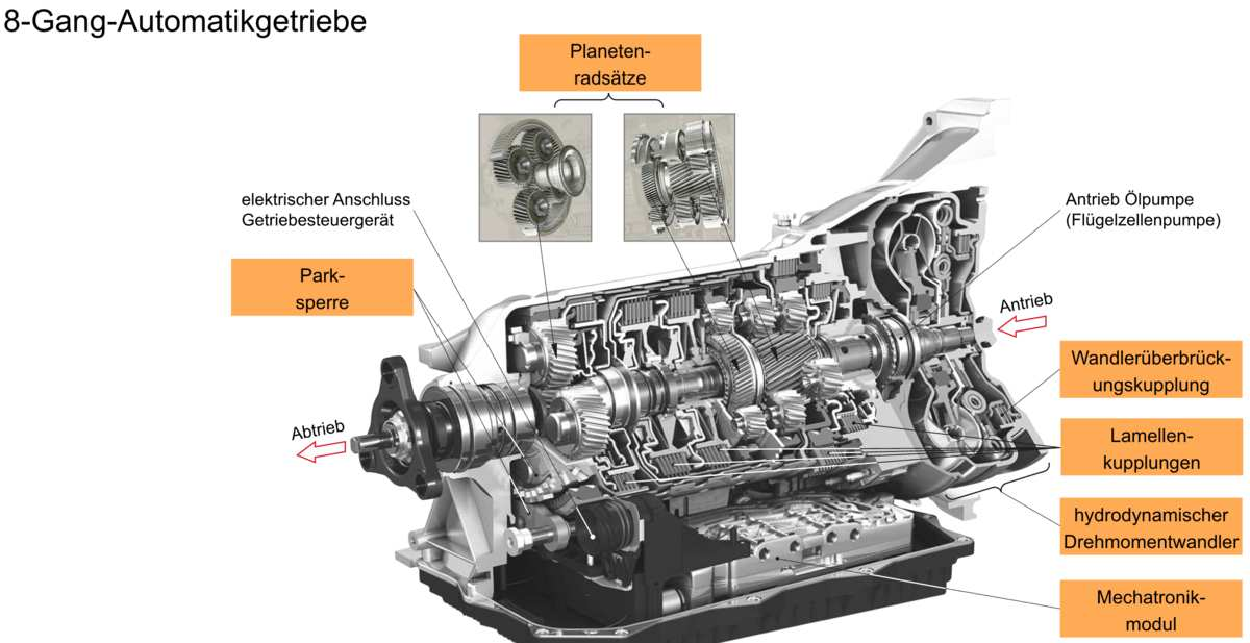
\includegraphics[width=0.7\textwidth]{images/Automatikgetriebe/Automatikgetriebe-1.pdf}
\caption{Automatikgetriebe, Quelle: Europa-Verlag}
%\label{fig:}%% anpassen
\end{figure}

\section{Fragen zum
Automatikgetriebe}\label{fragen-zum-automatikgetriebe}

\textbf{Aufgabe der Ölpumpe im Automatikgetriebe}

\begin{enumerate}
\item
  Wandler-Fülldruck
\item
  Schmierdruck für Planetengetriebe und Wandler
\item
  Arbeitsdruck zum Schalten der Lamellenkupplung
\end{enumerate}

\newpage

\textbf{Aufgabe eines hydrodynamischen Drehmomentwandlers}

\begin{enumerate}
\item
  Drehmoment wandeln und übertragen
\item
  Drehschwingungen vom Motor dämpfen
\item
  weiches und komfortables Anfahren ermöglichen
\end{enumerate}

\textbf{Überbrückungskupplung} Kraftfluss bei hohen Drehzahlen zwischen
Pumpenrad und Turbinenrad $\to$ Schlupf ausgleichen, Kraftstoff
sparen.

\textbf{Leitrad} bei unterer Drehzahl $\to$ Drehmomentverstärkung

\newpage

\textbf{Erklären Sie kurz gefasst die Wirkungsweise des hydrodynamischen
Drehmomentwandlers.}

\begin{figure}[!ht]% hier: !ht
\centering
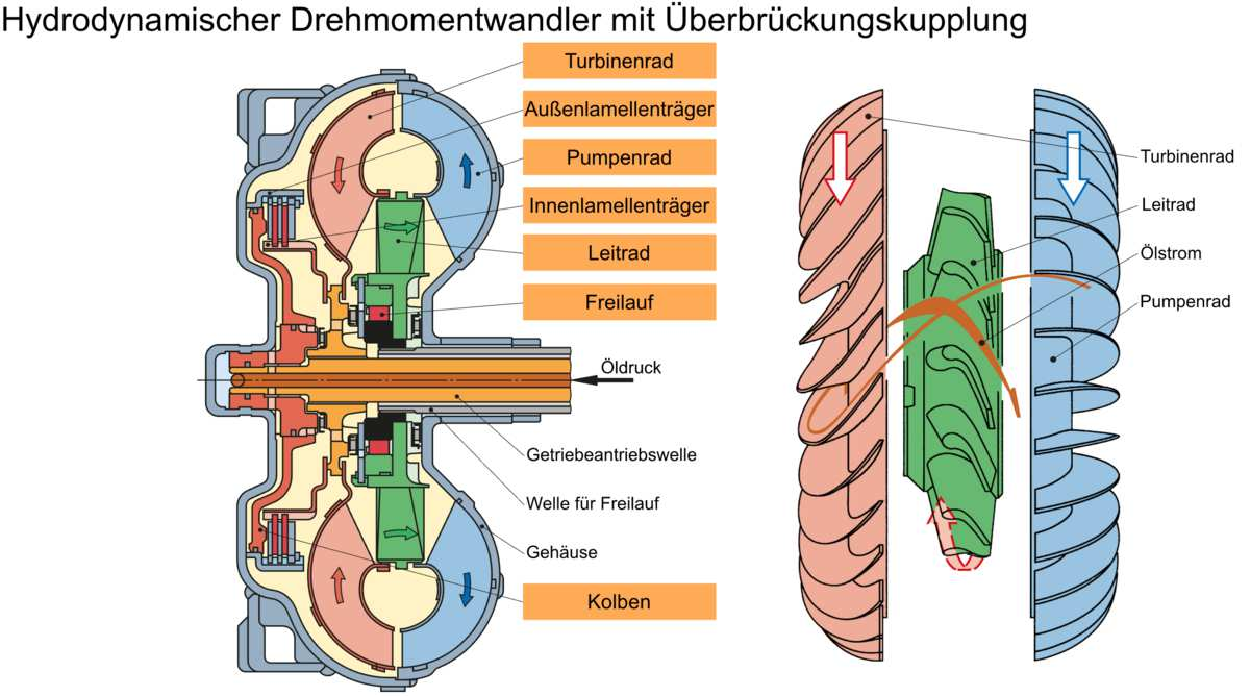
\includegraphics[width=0.7\textwidth]{images/Automatikgetriebe/Automatikgetriebe-2.pdf}
\caption{Hydrodynamischen Drehmomentwandler, Quelle: Europa-Verlag}
%\label{fig:}%% anpassen
\end{figure}

\begin{figure}[!ht]% hier: !ht
\centering
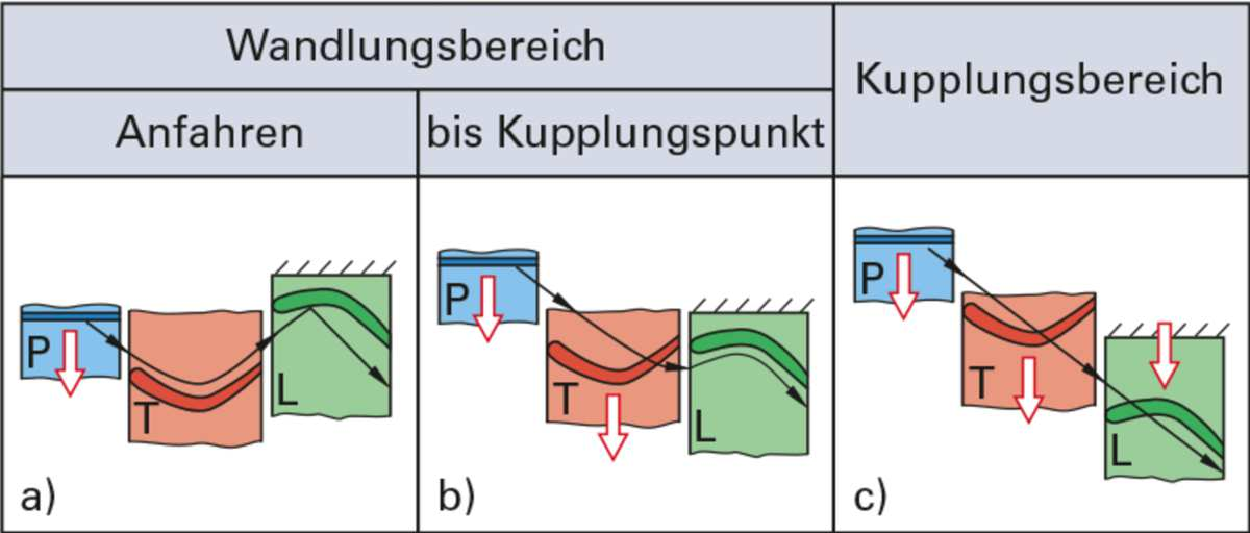
\includegraphics[width=0.4\textwidth]{images/Automatikgetriebe/Automatikgetriebe-3.pdf}
\caption{Drehmomentverstärkung, Quelle: Europa-Verlag}
%\label{fig:}%% anpassen
\end{figure}

\begin{table}[!ht]% hier: !ht 
\centering 
	\caption{}% \label{tab:}%% anpassen 
\begin{tabular}{@{}llll@{}}
\hline
\textbf{Wandlungsbereich} & \textbf{Anfahren} & \textbf{Kupplungspunkt}
& \textbf{Kupplungsbereich} \\
\hline
\textbf{Pumpenraddrehzahl} & Motordrehzahl & Motordrehzahl &
Motordrehzahl \\
\textbf{Turbinenraddrehzahl} & Null & Nimmt zu & > 85 \%
Pumpendrehzahl \\
\textbf{Leitraddrehzahl} & Null & Null & $\sim$ Turbinendrehzahl \\
\textbf{Ablenkwinkel des Ölstroms} & Groß & Klein & Keiner \\
\textbf{Drehmomenterhöhung} & Groß & Klein & Keine \\
\hline
\end{tabular} 
\end{table}

Je größer der Unterschied zwischen Pumpen- und Turbinenraddrehzahl,
desto größer ist die Drehmomenterhöhung.

\begin{figure}[!ht]% hier: !ht
\centering
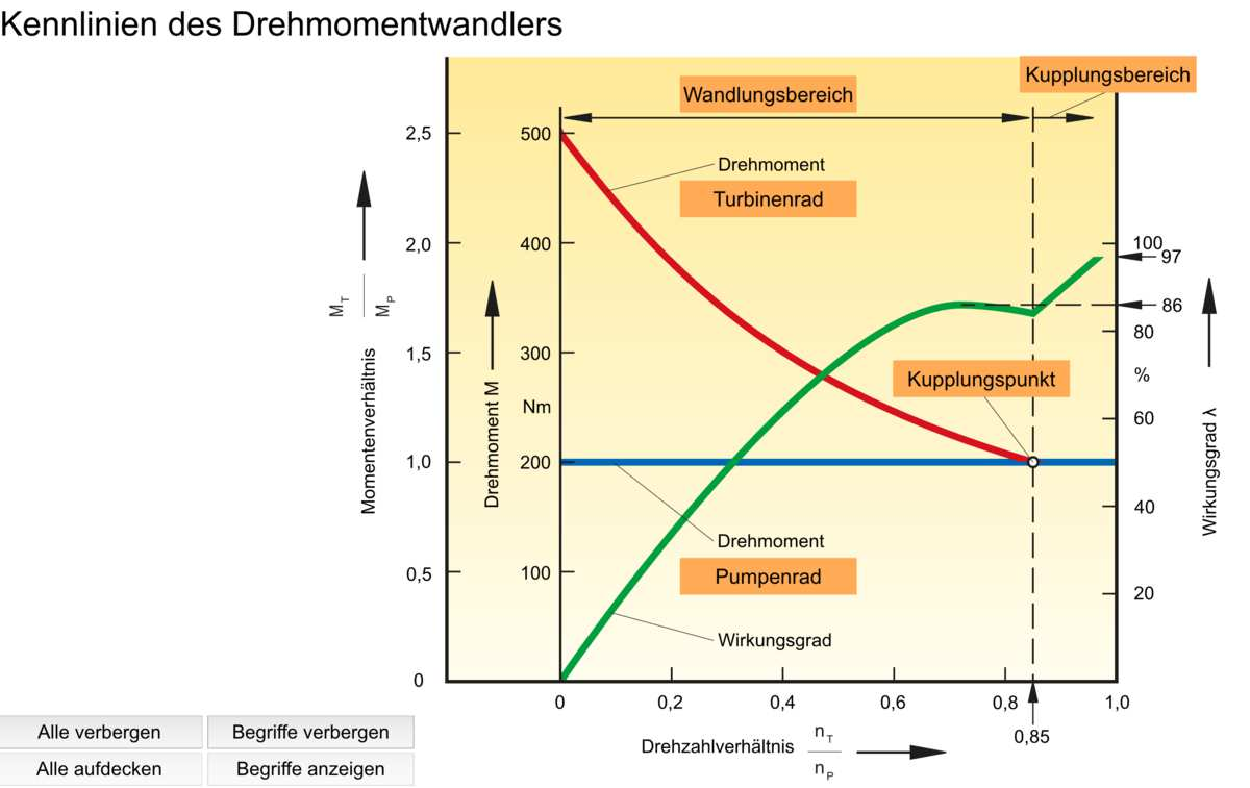
\includegraphics[width=0.7\textwidth]{images/Automatikgetriebe/Automatikgetriebe-4.pdf}
\caption{Kennlinien des Drehmomentwandlers, Quelle: Europa-Verlag}
%\label{fig:}%% anpassen
\end{figure}

Das Pumpenrad, mit der Motorkurbelwelle verbunden, versetzt das
Getriebeöl in strömende Bewegung. Das Turbinenrad, mit der
Getriebeeingangswelle verbunden, wird durch das strömende Getriebeöl
mitgenommen. Das Leitrad stützt sich über einen Freilauf entgegen der
Motordrehrichtung ab und lenkt den Ölstrom strömungsgünstig auf das
Pumpenrad zurück. Hierdurch kommt es zu einer Unterstützung des
Pumpenrades und damit zu einer Drehmomentverstärkung um bis zu 150 \%.
Die Drehmomentverstärkung ist proportional zur Drehzahldifferenz
zwischen Pumpen- und Turbinenrad. Beträgt die Drehzahl des Turbinenrades
etwa 85 \% der Drehzahl des Pumpenrades, ist der Kupplungspunkt
erreicht. Bei weiterem Drehzahlanstieg arbeitet der Wandler nur noch als
hydrodynamische Kupplung, weil sich das Leitrad durch den Freilauf
gelöst hat und frei mit dreht. Die Drehmomentverstärkung entfällt.

\textbf{Was versteht man unter der Festbremsdrehzahl bei einem
Automatikfahrzeug?}

\begin{itemize}
\item
  Es ist, die vom Hersteller angegebene Drehzahl, die ein Motor unter
  Volllaststellung am Fahrpedal bei eingelegter Fahrstufe und betätigter
  Betriebs- und Feststellbremse erreichen muss, ohne sie zu
  überschreiten. Die Prüfzeit darf max. 5 s betragen.
\item
  Mögliche Ursachen bei zu geringer Drehzahl:

  \begin{itemize}
  \item
    Wandlerfreilauf rutscht durch
  \item
    Störung im Motor (Keine Leistung)
  \end{itemize}
\item
  Mögliche Ursachen bei zu hoher Drehzahl:

  \begin{itemize}
  \item
    Wandler stellt keinen vollständigen Kraftschluss her (Ölstand?)
  \item
    Getriebe rutscht durch (Drehzahl Getriebeeingang prüfen)
  \end{itemize}
\end{itemize}

\newpage

\textbf{Wie werden Automatikgetriebe grundsätzlich geschaltet?}

\begin{itemize}
\item
  Automatikgetriebe werden grundsätzlich hydraulisch geschaltet. Das
  Schalten erfolgt durch das Schließen und Öffnen von Lamellenkupplungen
  und --bremsen, sowie, bei älteren Getriebevarianten, Bremsbändern.
\item
  Während ältere Getriebe oftmals hydropneumatisch in Abhängigkeit von
  Motordrehzahl (\textbf{Arbeitsdruck}), Last (\textbf{Modulierdruck})
  und Fahrgeschwindigkeit (\textbf{Reglerdruck}) gesteuert wurden,
  erfolgt die Steuerung heutzutage meistens elektronisch über die
  elektrohydraulische Steuereinheit. Hierbei werden bei der Definition
  der Schaltpunkte nicht nur die Hauptsteuergrößen Motordrehzahl, Last
  und Fahrgeschwindigkeit, sondern auch Nebensteuergrößen, wie z.B.
  Öltemperatur, Fahrertyp (sportlich, defensiv~\ldots),
  Betriebsbedingungen (Solo, Hängerbetrieb~\ldots), Eingriff
  Fahrdynamikregelung usw. berücksichtigt.
\end{itemize}

\newpage

\textbf{Aus welchen Teilen besteht der Planetenradsatz eines
Planetengetriebes und wie sind diese Teile angeordnet?}

\begin{figure}[!ht]% hier: !ht
\centering
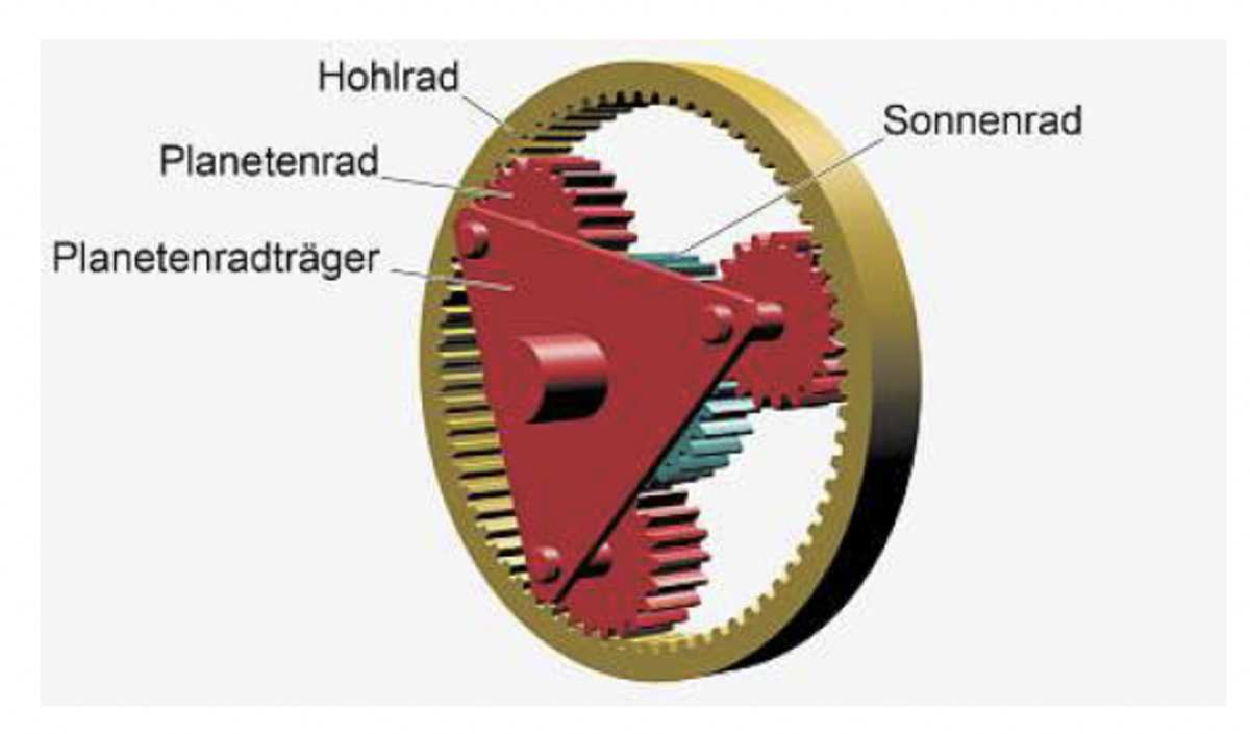
\includegraphics[width=0.3\textwidth]{images/Automatikgetriebe/Automatikgetriebe-6.pdf}
\caption{Planetenradsatz, Quelle: Europa-Verlag}
%\label{fig:}%% anpassen
\end{figure}

Zentrales Bauelement des einfachen Planetenradsatzes ist das Sonnenrad.
Auf diesem laufen Planetenräder, die ihrerseits durch den
Planetenradträger untereinander verbunden sind. Die Planetenräder werden
vom Hohlrad umschlossen, in welchem sie ebenfalls ablaufen können.

\textbf{Welchen Vorteil hat ein Planetengetriebe gegenüber einem
Schaltgetriebe?}

Es lässt sich unter Last schalten, d.h. zum Schalten ist keine
Trennkupplung zwischen Motor und Getriebe erforderlich.

\textbf{Was ist die Voraussetzung für die Kraftübertragung?}

\begin{enumerate}
\item
  Möglichkeit: 1x Antrieb (Antriebskupplungen), 1x fest gebremst
  (Bremskupplungen), 1x Abtrieb
\item
  Möglichkeit: 2x angetrieben, 1x Abtrieb
\end{enumerate}

\begin{figure}[!ht]% hier: !ht
\centering
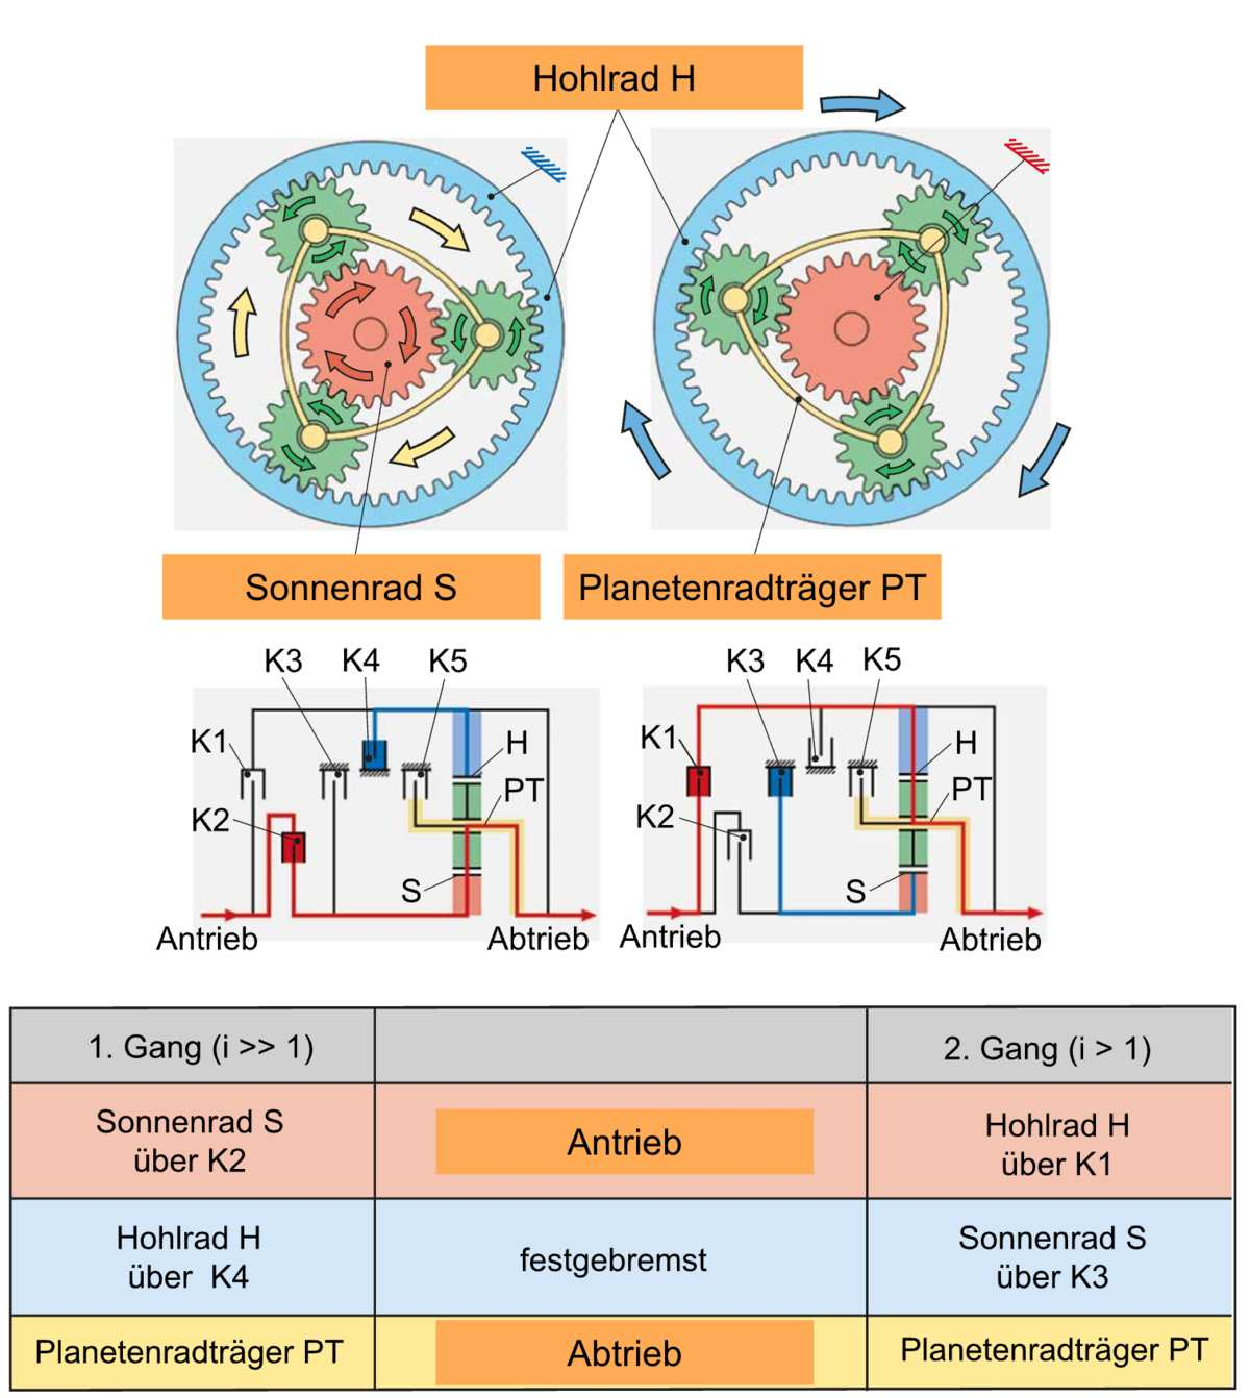
\includegraphics[width=0.4\textwidth]{images/Automatikgetriebe/Automatikgetriebe-5.pdf}
\caption{Kraftübertragung, Quelle: Europa-Verlag}
%\label{fig:}%% anpassen
\end{figure}

\newpage

\textbf{Worin unterscheiden sich die Planetengetriebe Simpson und
Ravigneaux?}

\begin{figure}[!ht]% hier: !ht
\centering
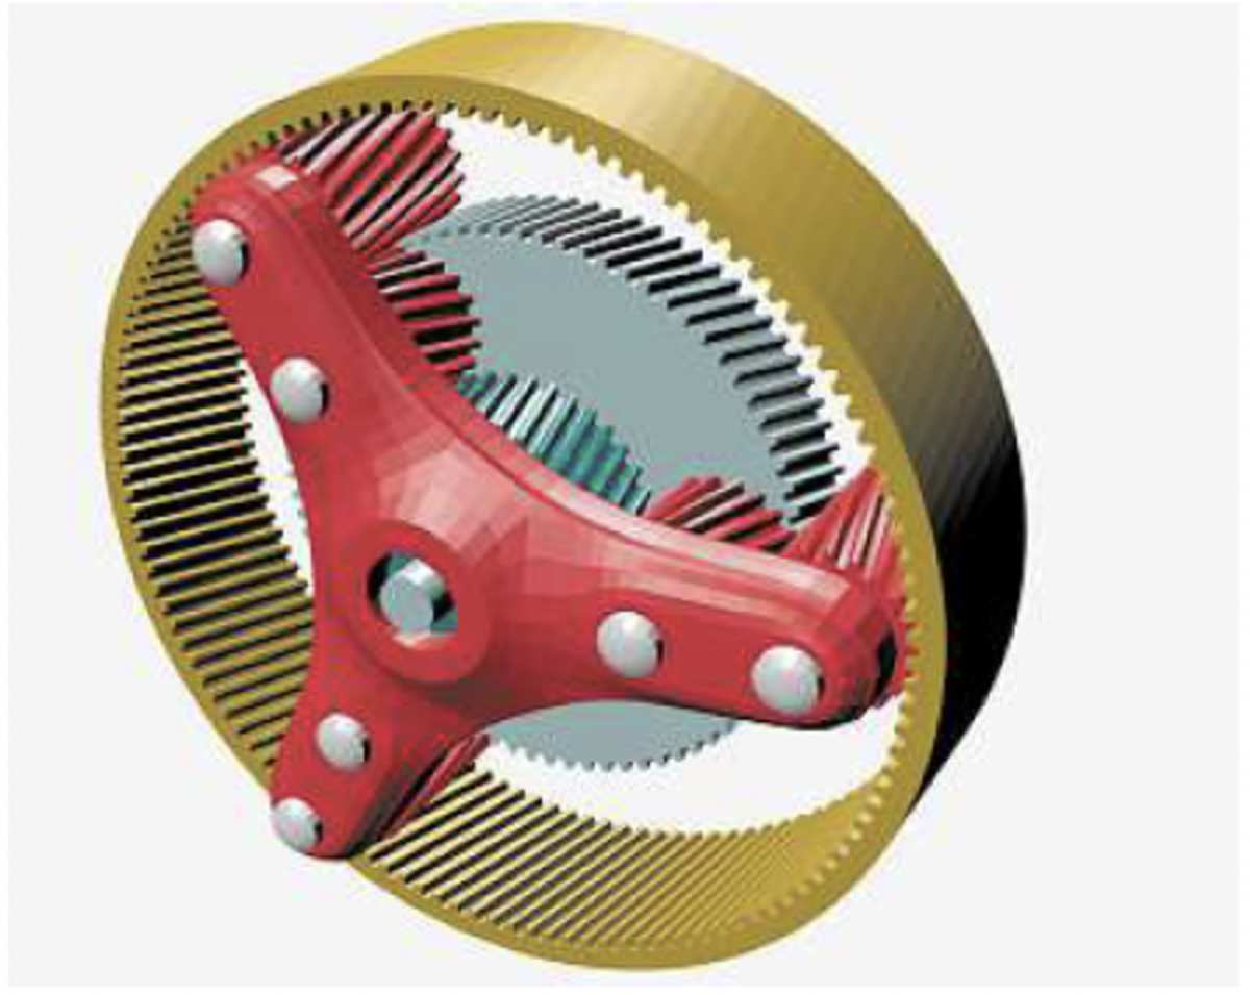
\includegraphics[width=0.3\textwidth]{images/Automatikgetriebe/Automatikgetriebe-7.pdf}
\caption{Ravigneaux-Planetengetriebe, Quelle: Europa-Verlag}
%\label{fig:}%% anpassen
\end{figure}

\begin{figure}[!ht]% hier: !ht
\centering
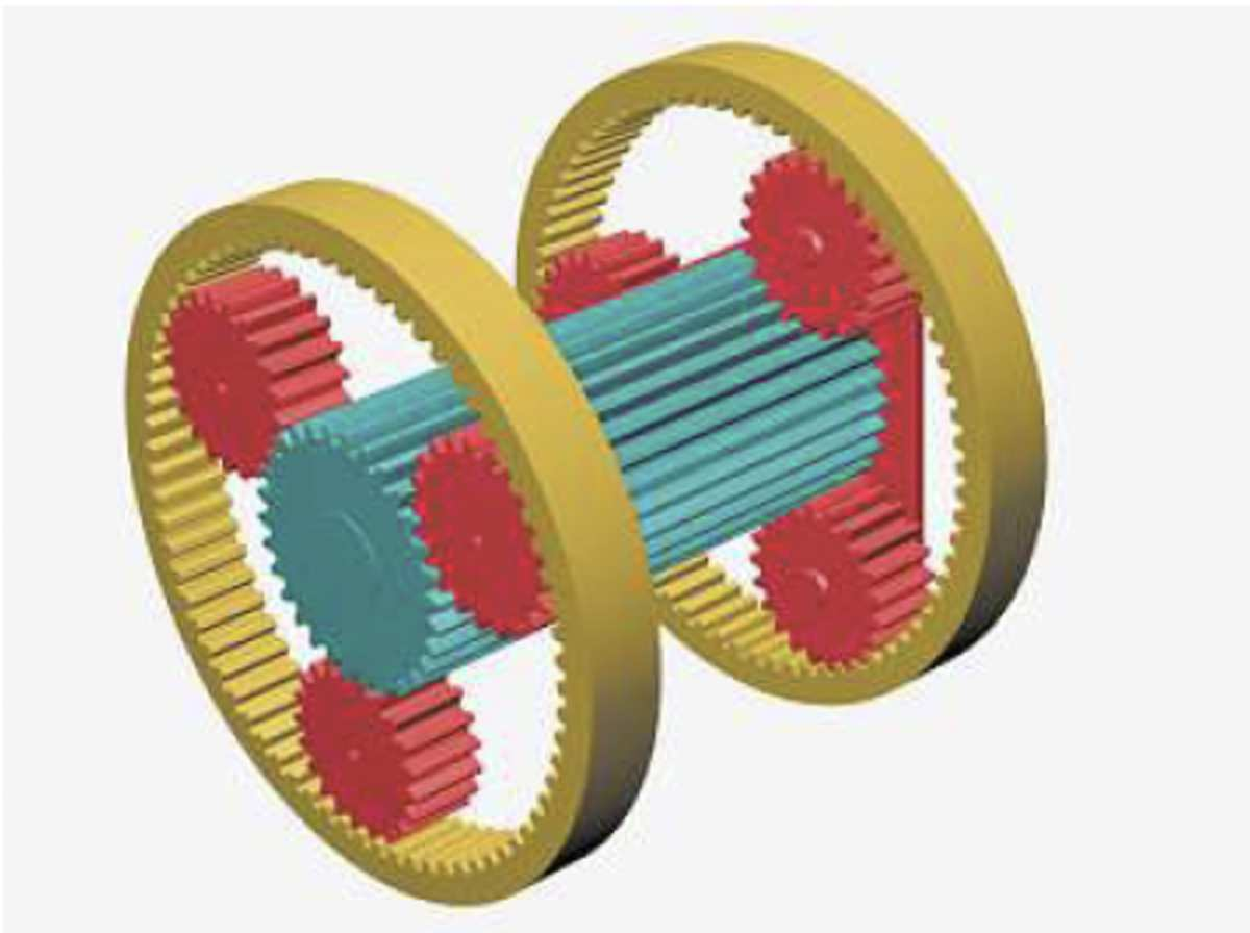
\includegraphics[width=0.3\textwidth]{images/Automatikgetriebe/Automatikgetriebe-8.pdf}
\caption{Simpson-Planetengetriebe, Quelle: Europa-Verlag}
%\label{fig:}%% anpassen
\end{figure}

\begin{itemize}
\item
  Das Simpson-Planetengetriebe besteht aus zwei Planetenradsätzen, die
  sich ein Sonnenrad teilen.
\item
  Beim Ravigneaux-Planetengetriebe teilen sich zwei Planetenradsätze ein
  gemeinsames Hohlrad.
\end{itemize}

\newpage

\textbf{Beschreiben Sie die Wirkungsweise einer Lamellenkupplung in
einem Automatikgetriebe.}

\begin{figure}[!ht]% hier: !ht
\centering
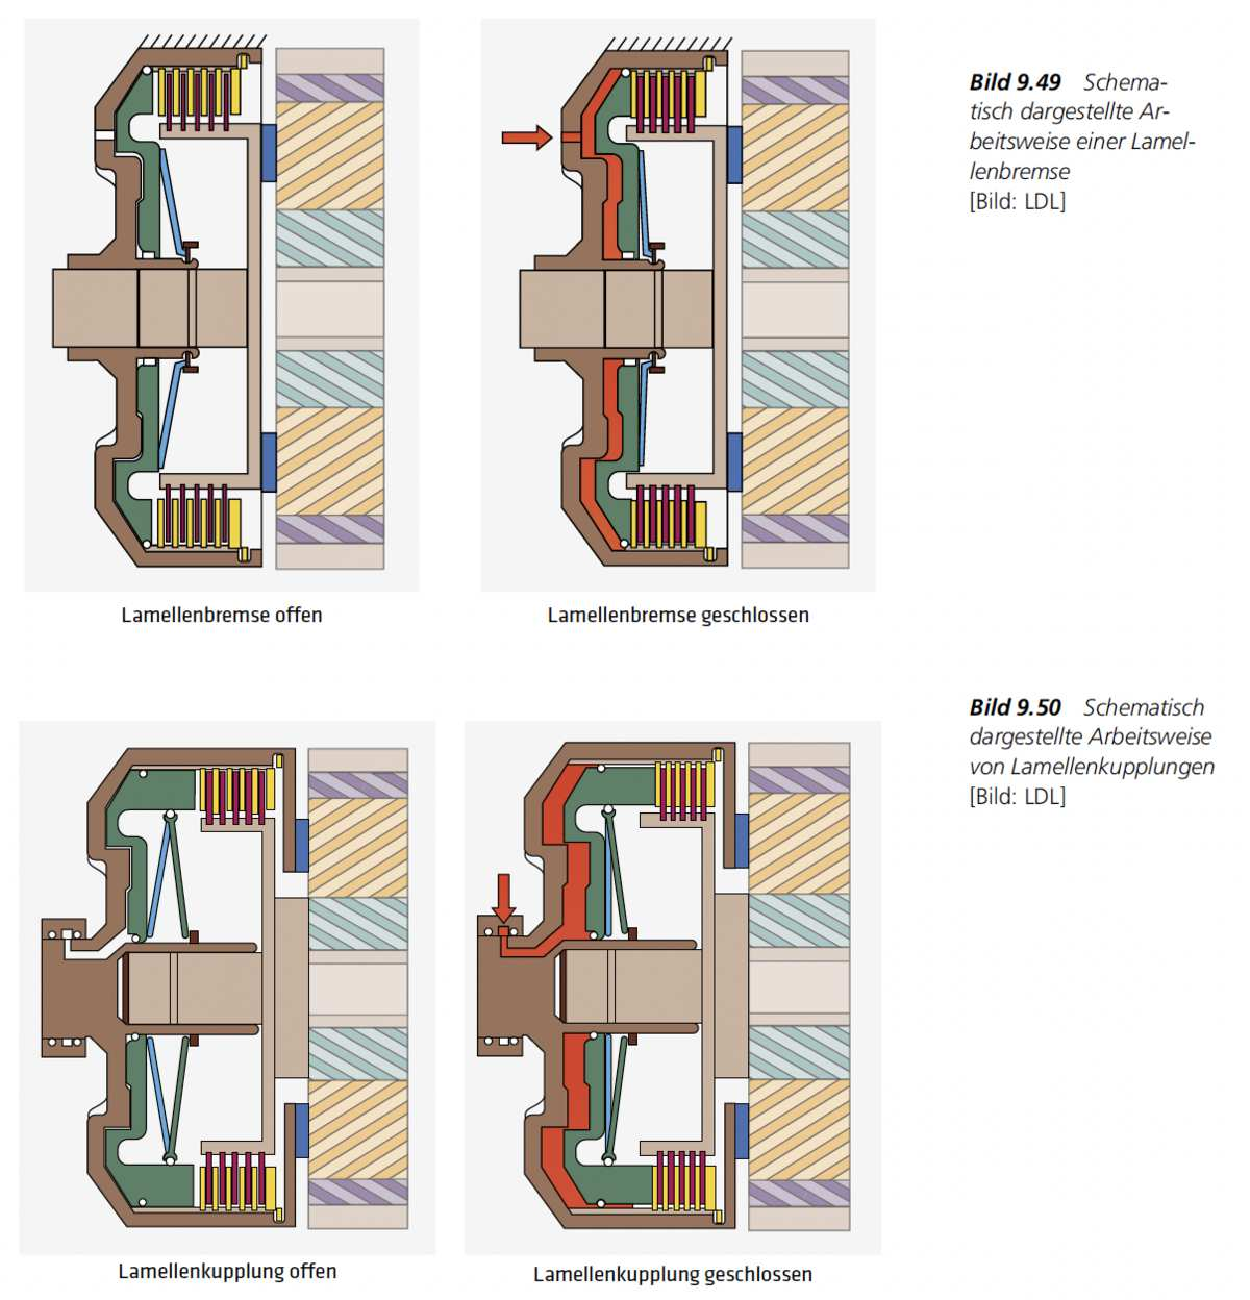
\includegraphics[width=0.7\textwidth]{images/Automatikgetriebe/Automatikgetriebe-12.pdf}
\caption{Lamellenkupplung, Quelle: Europa-Verlag}
%\label{fig:}%% anpassen
\end{figure}

Über eine beidseitig abgedichtete Wellenbohrung gelangt das Getriebeöl
unter Druck hinter den Kolben der Lamellenkupplung. Dieser fährt aus und
presst das Lamellenpaket, welches aus formschlüssig mit dem
Außenlamellenträger verbundenen Außenlamellen und formschlüssig mit dem
Innenlamellenträger verbundenen Innenlamellen besteht zusammen. Beide
Bauteile werden nun kraftschlüssig und drehen sich gleichmäßig oder mit
definiertem Schlupf. Zum Lösen der Kupplung wird der Druck abgebaut,
wodurch der Kolben mithilfe einer Tellerfeder in die Ausgangslage
gedrückt wird. Um zu verhindern, dass es durch das, der Fliehkraft
ausgesetzte Öl im Kolbenraum zu einer Betätigung der Kupplung kommt,
gibt es vor dem Kolben eine Kolbenabdeckung, die als Gegenkolben wirkt
und die Ruhelage des Kolbens sicherstellt.

\newpage

\textbf{Wozu dienen die 1. und falls vorhanden, die 2. Ölpumpe im
Automatikgetriebe?}

\begin{enumerate}
\item
  Aufgaben der 1. Ölpumpe

  \begin{itemize}
  \item
    Befüllung des Wandlers oder der Kupplung mit Getriebeflüssigkeit
  \item
    Schmierölversorgung der Planetengetriebe
  \item
    Belieferung der Steuereinheit mit, unter Druck stehendem Getriebeöl
  \item
    Betätigung der Lamellenkupplungen und -bremsen
  \end{itemize}
\item
  Aufgabe der 2. Ölpumpe

  \begin{itemize}
  \item
    Schmierölversorgung beim Abschleppen
  \end{itemize}
\item
  Aufgabe der elektrischen Ölpumpe

  \begin{itemize}
  \item
    Druckerhalt im Getriebe im Start-Stopp-Betrieb
  \end{itemize}
\end{enumerate}

\textbf{Wie ist die Wirkungsweise einer Parksperre?}

\begin{figure}[!ht]% hier: !ht
\centering
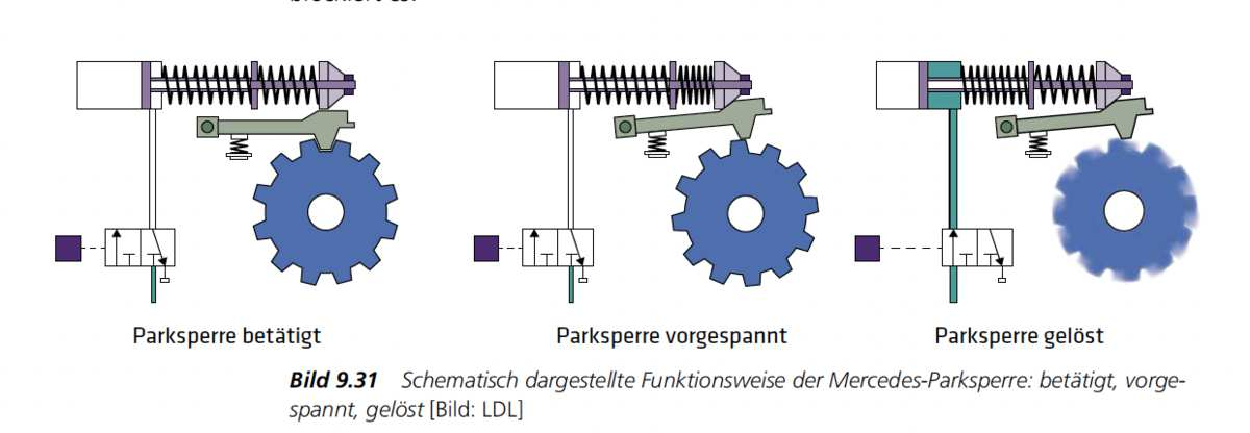
\includegraphics[width=0.7\textwidth]{images/Automatikgetriebe/Automatikgetriebe-9.pdf}
\caption{Parksperre, Quelle: Europa-Verlag}
%\label{fig:}%% anpassen
\end{figure}

Bei Betätigung des Wählhebels in Stellung >>P<<, wird über ein Gestänge,
einen Bowdenzug oder einen Stellmotor, eine mechanische Sperrklinke
freigegeben, die sich in das, mit der Getriebeabtriebswelle verbundene
Parksperrenrad einhakt und so die Getriebeabtriebswelle blockiert.

\textbf{Was versteht man unter einer adaptiven elektrohydraulischen
Getriebesteuerung?}

Darunter versteht man die Anpassung der elektrohydraulischen
Getriebesteuerung an die Einsatzbedingungen des Fahrzeugs, den Fahrstil
des Fahrers und den Verschleiß im Getriebe. Das Steuergerät ist
selbstlernend und passt die Schaltzeitpunkte und die Drücke im Getriebe
so an, dass eine konstant hohe Schaltqualität gewährleistet werden kann.

\textbf{Lassen sich Fahrzeuge mit einem vollautomatischen Getriebe
anschleppen?}

Das Anschleppen ist im Normalfall nicht möglich, da zum Schalten der
Gänge hydraulischer Druck erforderlich ist. Da der Motor nicht läuft,
fördert auch die 1. Ölpumpe nicht. Die Ausnahme besteht bei
Automatikgetrieben mit 2. Ölpumpe, die von der Getriebeabtriebswelle
angetrieben wird.


	%%%%%%%%%%%%%%%%%%%%%%%%%%%%%%%%%%%%%%%%%%%%%%%%%%%%%%%%%%%%%%%%%%
    % Bibliographie
    \printbibliography[category=cited]
\end{document}
